\chapter*{Background}
\addcontentsline{toc}{chapter}{Background}
\section{Literature Review}
In order to understand the design requirements of the library, a literature review needed to be performed. The scope was
narrowed down to 3 systems that showed promise and were broadly representative of the antenna configuration that future
systems would adopt. Most systems will adopt one of the following setups
\begin{enumerate}
    \item Monostatic
    \item Leveled Multistatic
    \item Fully Multistatic
\end{enumerate}
\noindent These terms relate to the position of antennas around the breast tissue and how the resulting scan data would
be structured. \hfill \break

\subsection{MARIA M4}
The first system we will look at is the MARIA M4 system developed by Preece et al within the Electrical and Engineering
Department of the University of Bristol \cite{preeceMARIAM4Clinical2016}. This is the 4th iteration in a series of MARIA systems that evolved from a
system of 16 UWB antennas to 60 antennas in the current system. These all operate in a multistatic configuration,
meaning that any antenna in the array can listen to any other antenna in the array, an example of which can be seen in
Figure \ref{fig:MultistaticExample}. This figure shows a top-down view, however, one can imagine this being generalized
to a hemisphere of antennas around the breast. \hfill

\begin{figure}
    
\includegraphics[width=0.4\textwidth]{multistaic.png}
    \centering
    \caption{Example of a Fully Multistatic Configuration (Top-Down)}
    \label{fig:MultistaticExample}
\end{figure}

\noindent As stated before, the MARIA M4 systems makes use of the UWB spectrum over a frequency range of 3 to 8 GHz. A
VNA was used to step through the frequencies and collect the scans from the antenna. The system exploits the inherent
symmetry in the antenna reciprocity to halve the number of channels (made of a transmitting and receiving antenna)
collected, thereby speeding up the scan time. For the MARIA M4 system, this equates to a 1770 reduction in the number of
channels collected. Figure \ref{fig:MARIAM4}, shows the antenna array used in the M4 system (a), as well as the M5
system (c) which is an integrated package.


\begin{figure}
    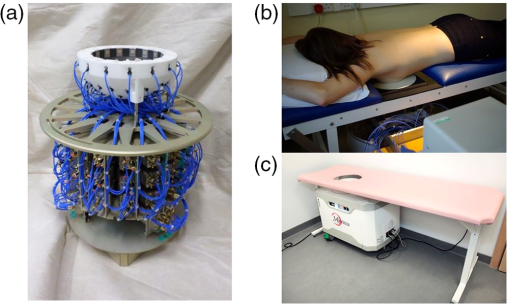
\includegraphics[width=0.5\textwidth]{MARIA_M4.png}
    \centering
    \caption{The MARIA M4 and M5 system. (a) The MARIA M4 antenna array. (b) The M4 in a clinical setting. (c) The integrated M5 package}
    \label{fig:MARIAM4}
\end{figure}

\noindent While the patient size was relatively small ($n = 86$) the system did show promise. The machine showed a
sensitivity of 74\% when compared with the "gold-standard' of an ultrasound.  